\documentclass{article}

\usepackage[a4paper,left=2.5cm,right=2.5cm,top=2.5cm,bottom=2.5cm]{geometry}
\usepackage[bahasa]{babel}

\usepackage{lipsum}
\usepackage{graphicx}
\usepackage{hyperref}
\usepackage{tikz}
% \usepackage{biblatex}
% \addbibresource{main.bib}
\usepackage{apacite}
\usepackage{longtable}
% \usepackage[backend=biber,style=apa,citestyle=apa,sorting=ynt]{biblatex}
% \addbibresource{main.bib}
\usepackage{usebib}

\bibinput{main}
\graphicspath{ {./images/} }
\title{Tugas SPK}
\author{Ilman Samhabib 91122010\\62/MMSI/SIB}
\date{\today}

\begin{document}

% \maketitle
% \titlepage
% \newpage
% \tableofcontents
% \newpage
\begin{center}
    Tugas SPK
    \\ Tema: \textbf{Programmatic Advertising} 
    \\ 991122010 62/MMSI/SIB
    \\ Ilman Samhabib
\end{center}

\subsubsection*{Nomor 1}
Deskripsikan jumlah atribut/field yang anda gunakan pada dataset. Beri penjelasan pada masing masing dataset
\bigbreak
\begin{center}
    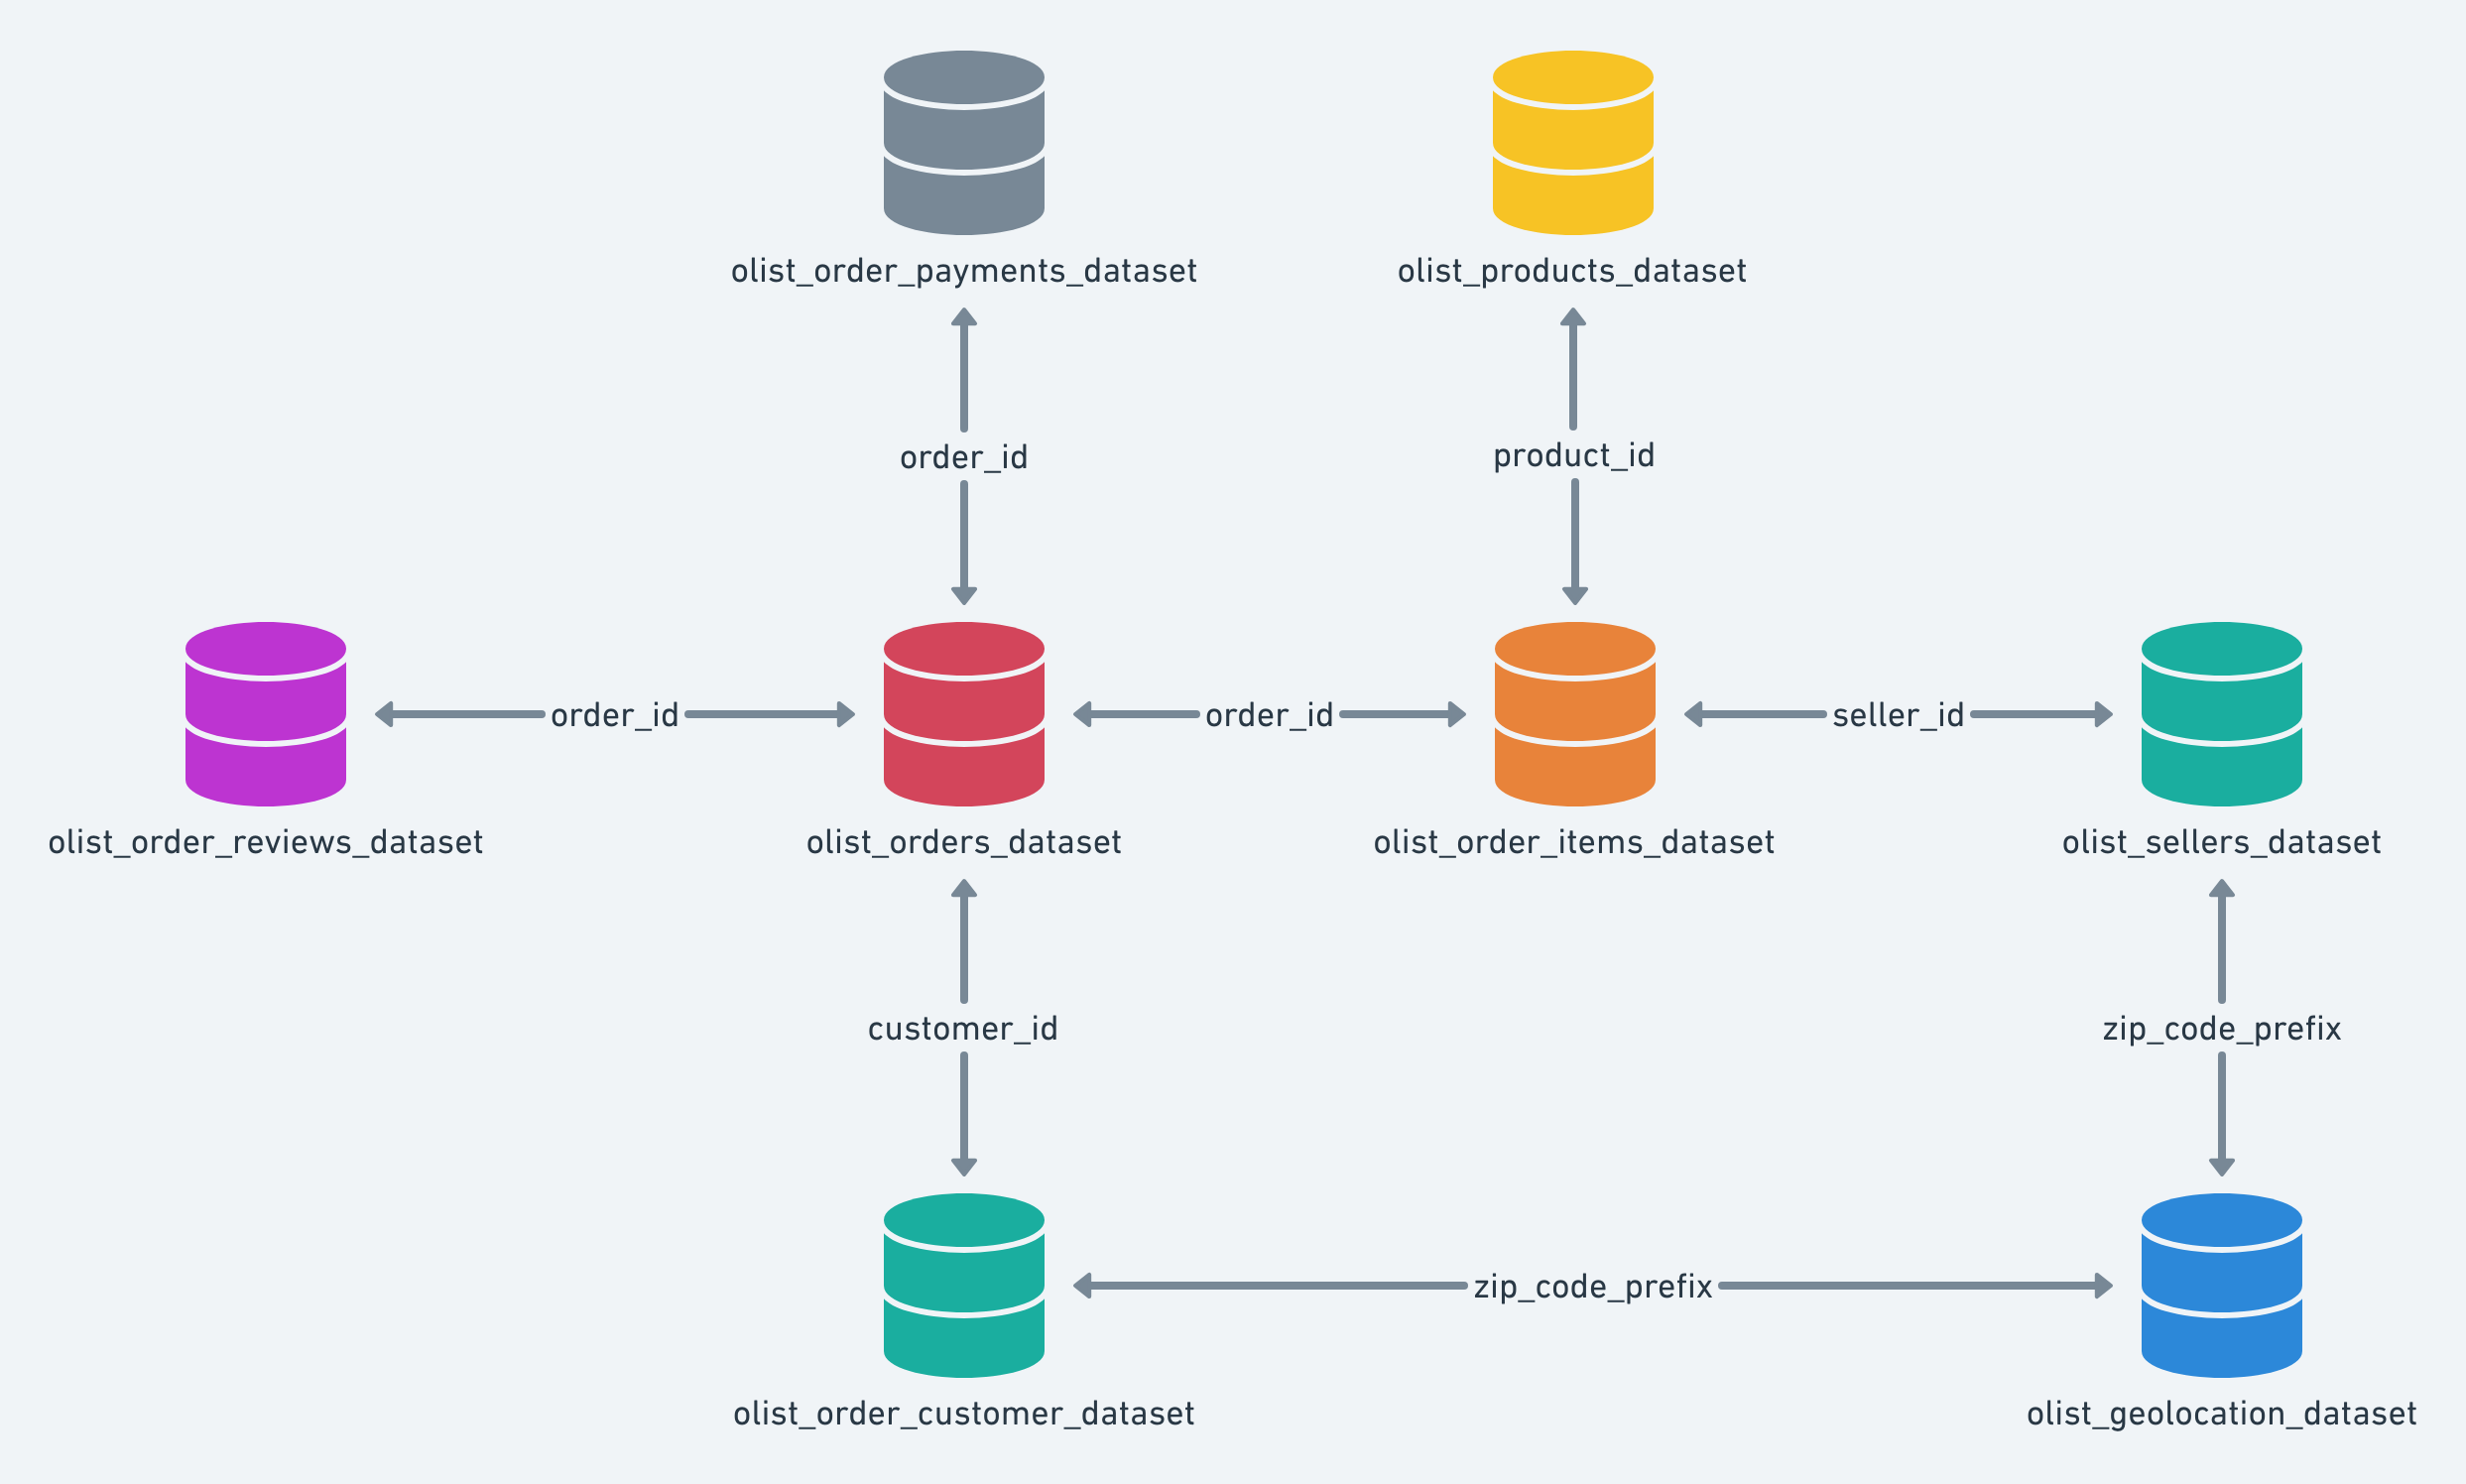
\includegraphics[width=11cm, height=9cm]{images/olist.png}
\end{center}
Data set yang digunakan dataset olist Brazilian E-commerce \cite{Olist_2018}, 
(\url{https://www.kaggle.com/datasets/olistbr/brazilian-ecommerce})
berisi data order pada tahun 2017 yang terdiri dari beberapa file csv. Dataset dijoin dari beberapa tabel berbeda. 

Untuk kasus yang akan dijelaskan nanti pada soal ke tiga, akan diambil hanya beberapa fitur yaitu:
\\Price : Harga Barang Yang dipesan
\\Freight Value : Bea Import/Export 
\\Customer State : Provinsi Pelanggan
\\Seller State :Provinsi Penjual
\\Customer City : Provinsi Konsumen
\\Seller City : Kota Penjual

setelah di lakukan pembuangan data yang mengandung NaN data yang tersisa adalah sekitar 11000an baris

\subsubsection*{Nomor 2}
Pola apa yang bisa anda angkat sebagai masalah 
penelitian dari dataset yang anda dapatkan?
\bigbreak
disini akan diangkat masalah mengenai memprediksi review apakah bintang 1, 2 ,3 ,4 atau 5, 
\subsubsection*{Nomor 3}
Berdasarkan beberapa literature review yang anda baca, 
metode apa yang anda gunakan dalam menyelesaikan maslah pada dataset. 
Apa alasan menggunakan metode tersebut
\bigbreak
disini akan digunakan klasifikasi dengan decision tree, 
akan dicoba beberapa jenis implementasi model decision tree (DecisionTreeClassifier(CART),RandomForestClassifier,XGBoost) dan juga selain tree, KNeighborsClassifier
\\
decision tree dan KNeighbor dipilih karena dapat cepan 
untuk meneyelesaikan fitting, sedangkan algoritma lain terlalu lama dijalankan di dalam komputer yang saya gunakan 
\subsubsection*{Nomor 4}
Buat simulasinya dengan menggunakan tools datamining
 \bigbreak
 di sini digunakan jupyter notebook
 \\
 \begin{center}
    Decision Tree(CART)   
 \end{center}
  \begin{center}
    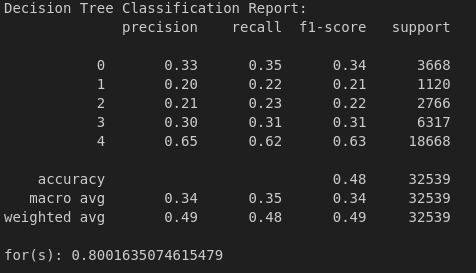
\includegraphics[width=8cm, height=7cm]{images/decision-tree-f1.png}
    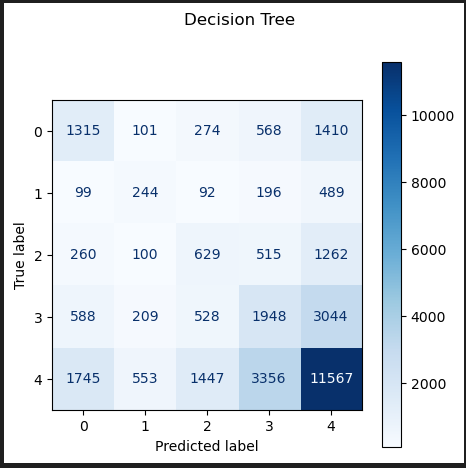
\includegraphics[width=8cm, height=7cm]{images/Dt-confusion.png}   
 \end{center}
 \begin{center}
    KNN(5,uniform)
 \end{center}
 \begin{center}
    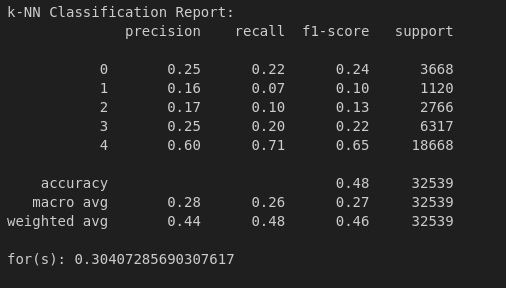
\includegraphics[width=8cm, height=7cm]{images/knn-f1.png}
    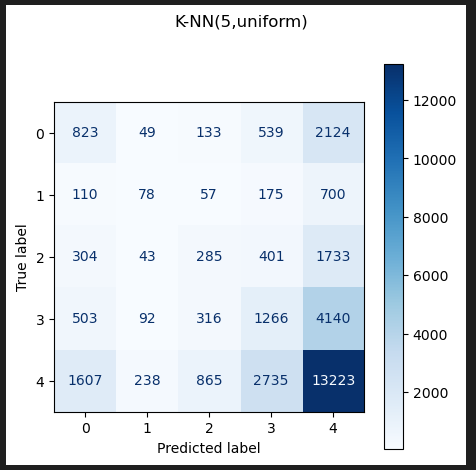
\includegraphics[width=8cm, height=7cm]{images/knn-confusion.png}
 \end{center}
 \begin{center}
    Random Forest
 \end{center}
 \begin{center}
    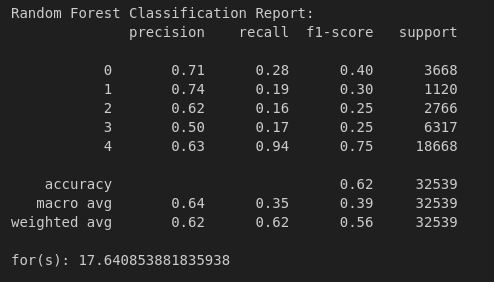
\includegraphics[width=8cm, height=6cm]{images/random-forest-f1.png}
    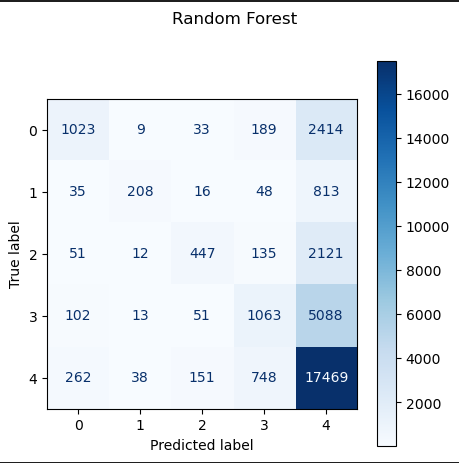
\includegraphics[width=8cm, height=6cm]{images/rf-confusion.png}
 \end{center}
 \begin{center}
    XGBoost
 \end{center}
 \begin{center}
    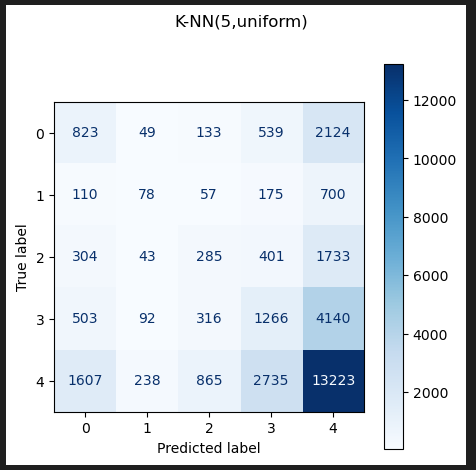
\includegraphics[width=8cm, height=6cm]{images/knn-confusion.png}
    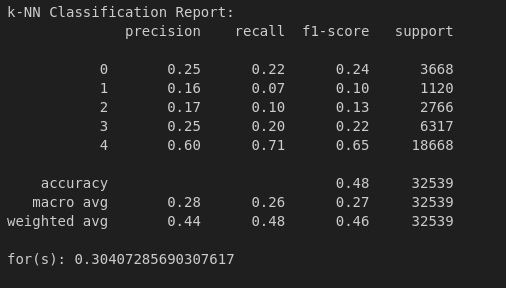
\includegraphics[width=8cm, height=6cm]{images/knn-f1.png}
 \end{center}

\subsubsection*{Nomor 5}
Apa yang bisa anda simpulkan dari kesuluruhan proses yang anda lakukan menggunakan dataset dan metode yang anda purpose.
\begin{enumerate}
    \item Karena dataset yang tidak \emph{balanced} pada fitur sasaran, kebanyakan model yang dihasilkan dapat memprediksi fitur review bintang 5, dan untuk bintang lainnya urang tepat
    \item model yang lebih simple dapat diselesaikan komputer dengan lebih cepat
\end{enumerate}




\bibliographystyle{apacite}
\bibliography{main}
% \printbibliography


\end{document}